\documentclass[11pt]{article}
\usepackage[preprint]{acl}

\usepackage{times}
\usepackage{latexsym}
\usepackage[T1]{fontenc}
\usepackage[utf8]{inputenc}
\usepackage{microtype}
\usepackage{inconsolata}
\usepackage{graphicx}
\usepackage{float}
\usepackage{booktabs}
\usepackage{array}
\usepackage{tabularx}
\usepackage{makecell}
\usepackage{amsmath}
\usepackage{amssymb}
\usepackage{xspace}
\usepackage{url}
\usepackage{xcolor}
\usepackage{listings}
\usepackage{enumitem}
\usepackage{subcaption}

\lstset{
  basicstyle=\ttfamily\scriptsize,
  columns=fullflexible,
  breaklines=true,
  frame=single,
  xleftmargin=0.5em,
  xrightmargin=0.5em
}

\title{Who Judges the Judge in RAG?\\ Controlled Pairing Effects in LLM Evaluation of Induced Factual Errors}

\author{Sriram Selvam\\
  \texttt{selvamsriram@gmail.com}
  \And
  Anneswa Ghosh\\
  \texttt{anneswaghosh@gmail.com}}

\newcommand{\method}{Eval-Pair Matrix\xspace}
\newcommand{\pp}{\ensuremath{\mathrm{pp}}\xspace}
\newcommand{\model}[1]{\textsc{#1}}
\newcolumntype{Y}{>{\raggedright\arraybackslash}X}
\newcolumntype{L}[1]{>{\raggedright\arraybackslash}p{#1}}

\begin{document}
\maketitle

\begin{abstract}
LLM-as-a-judge evaluation is now common for retrieval-augmented generation (RAG), yet the judge is often the same model family as the system being evaluated. We introduce an \method protocol for RAG factuality: starting from GaRAGe questions and grounding passages, we create hidden, globally consistent factual perturbations, ask three LLM families to answer from the perturbed grounding, and then ask three LLM judges to evaluate those answers against the unmodified grounding. The judge sees only the question, candidate answer, and original passages; it never sees the perturbation or gold label. We audited the committed JSONL data directly with a new raw-data script. Across 300 balanced records, 897 labeled generator outputs, and 2,683 judge verdicts in a full $3\times3$ judge-by-generator matrix, generators follow perturbed evidence about half the time while rarely overriding retrieval with parametric memory (1--3\%). Judges detect induced factual errors with F1 between 79.9\% and 88.6\%. Same-model bias is not a single scalar: the aggregate diagonal-vs-off-diagonal F1 gap is only +0.8\pp, but GPT is recall-lenient on its own outputs, Gemini is stricter on its own outputs, and Grok is noisier on its own outputs. These opposing signatures cancel in aggregate. RAG evaluation should report the full judge-by-generator matrix, not only a pooled ``LLM judge'' score or an averaged same-model effect.
\end{abstract}

\section{Introduction}

Retrieval-augmented generation (RAG) systems combine a language model's parametric knowledge with external passages supplied at inference time \citep{lewis2020rag}. This makes them attractive for knowledge-intensive applications, but also creates a tension: the model may follow retrieved evidence that contradicts either its parametric memory or the original authoritative source. In practice, RAG answers are increasingly evaluated by another LLM rather than by humans, because LLM judges are cheap, fast, and can emit structured rationales \citep{liu2023geval,zheng2023judging,kim2023prometheus}. If the generator and judge are the same model, or from the same family, evaluation may become circular.

Existing LLM-as-a-judge work documents position, verbosity, length, style, familiarity, and self-preference effects \citep{zheng2023judging,dubois2024length,liu2024narcissistic,wataoka2024selfpreference,ye2024justice,spiliopoulou2025playfavorites}. But in open-ended preference settings, self-preference is hard to separate from true answer quality: a judge may prefer its own model because those answers are better, clearer, or more stylistically familiar. We study the question in a controlled factual setting. If we can induce a known factual error that is hidden from the judge, then the judge is not choosing a favorite answer; it is detecting whether a candidate answer contradicts original source passages.

We build this controlled task from GaRAGe, a RAG benchmark with human-written answers and passage-level grounding annotations \citep{sorodoc2025garage}. For each selected example, an LLM perturber chooses one answer-causal atomic claim and rewrites every passage that states or entails that claim so that the evidence consistently supports a plausible but false value. Generators answer the original question using this perturbed grounding. Judges then evaluate the generated answer against the original grounding only. The judge is blind to perturbation metadata, gold labels, and generator behavior labels.

The resulting object is an \method: rows are judges, columns are generators, and each cell reports factual-error detection precision, recall, F1, and localization. This design lets us measure whether diagonal cells, where judge and generator are the same display family, differ from off-diagonal cells while keeping question set, original sources, perturbation targets, and gold labels fixed.

\paragraph{Contributions.}
First, we introduce a controlled RAG factuality protocol that turns LLM-judge bias into a hidden-label error-detection problem. Second, we build a 300-record balanced perturbation set from GaRAGe and run three generator families and three judge families over it. Third, we audit the raw committed JSONL data with a new script rather than relying on summary markdown files. Fourth, we provide concrete examples and schemas for perturbation, validation, generation, behavior labeling, and judging. Fifth, we show empirically that same-model effects are heterogeneous: GPT is self-lenient in recall, Gemini is self-strict in recall, and Grok degrades on its own outputs. This is a more realistic conclusion than claiming a universal self-favoring or self-penalizing tendency.

\begin{figure*}[t]
  \centering
  
\includegraphics[width=0.99\linewidth]{figures/pipeline_big.pdf}
  \caption{The \method pipeline. Perturbations are generated and validated before answer generation. Judges see only the question, generated answer, and original grounding; perturbation metadata and gold labels are hidden from the judge. Rendered deterministically from Graphviz DOT.}
  \label{fig:pipeline}
\end{figure*}

\section{Related Work}

\paragraph{RAG and grounding evaluation.}
RAG was introduced as a way to combine parametric model memory with retrieved non-parametric evidence \citep{lewis2020rag}. Later work shows that models do not always use context robustly; relevant evidence can be missed when placed in the middle of a long context \citep{liu2023lost}. GaRAGe is a useful base for our study because it includes human-curated long-form answers and passage-level grounding annotations for 2,366 questions and more than 35K passages \citep{sorodoc2025garage}. Automated RAG evaluators such as RAGAS and ARES score dimensions like context relevance, answer faithfulness, and answer relevance; ARES further uses synthetic data, lightweight judges, and prediction-powered inference with a small human set \citep{es2023ragas,saadfalcon2023ares}. Our work is narrower but more controlled: rather than measuring general RAG quality, we generate paired original/perturbed grounding sets so that factual errors are known and localized.

\paragraph{RAG hallucination and factuality datasets.}
RAG does not eliminate hallucination: models can still make claims unsupported by retrieved content, misread retrieved evidence, or combine incompatible sources. RAGTruth addresses this by collecting nearly 18K naturally generated RAG responses with case-level and word-level hallucination annotations across domains \citep{niu2023ragtruth}. SelfCheckGPT uses sampling consistency to detect hallucinations in black-box generative models without external resources \citep{manakul2023selfcheckgpt}. FaithBench constructs challenging modern summarization hallucination cases on which popular detectors disagree \citep{bao2024faithbench}. These benchmarks are complementary. They study naturally occurring hallucinations or detector robustness, while our positive labels come from deliberately induced, hidden source perturbations that make the factual contradiction local and auditable.

\paragraph{LLM-as-a-judge evaluation.}
LLM judges have become common for NLG, instruction following, dialogue, and long-form response evaluation. G-Eval uses GPT-4 with task rubrics and form filling to improve agreement with human ratings \citep{liu2023geval}; MT-Bench and Chatbot Arena evaluate chat assistants using strong LLM judges and human preference comparisons \citep{zheng2023judging}; Prometheus trains an open evaluator to follow fine-grained rubrics \citep{kim2023prometheus}. These works motivate LLM judges but also expose artifacts. We do not ask the judge to assign a general quality score or preference. We ask for a binary factual-error decision and a source passage, with hidden gold labels constructed from controlled corruptions.

\paragraph{Judge bias, self-preference, and controls.}
Several studies ask whether models favor their own outputs. \citet{liu2024narcissistic} find that LM-based metrics can inflate scores for outputs from similar models. \citet{wataoka2024selfpreference} connect GPT-4 self-preference to familiarity and perplexity. \citet{spiliopoulou2025playfavorites} propose a statistical procedure to estimate self-bias while controlling for quality differences. \citet{ye2024justice} catalog multiple biases in LLM-as-a-judge settings, while length and position-bias studies show that surface artifacts can influence automatic judges \citep{dubois2024length,shi2024position}. Our contribution is complementary: because every positive case is an induced factual error against original evidence, the matrix measures error detection rather than preference. The resulting finding is also less one-dimensional than prior self-preference framing: one judge is descriptively self-lenient, one self-strict, and one noisier on self.

\section{Task and Data Construction}

\subsection{Base Dataset and Filtering}

We use GaRAGe as the base corpus. Each original example includes a question, a human-written answer, and grounding passages with annotations such as whether a passage answers the question. The pipeline first filters examples by five deterministic gates: valid question, information-seeking question, no false premise, validated answer, and at least two grounding passages labeled \texttt{ANSWER-THE-QUESTION}. A stratified sample of 300 records is frozen as the initial experimental pool.

\subsection{Perturbation Design}

For each question, an LLM perturber receives the question, the human answer, and the answer-bearing plus related grounding passages. The perturber must select exactly one answer-causal atomic value that is present in both the answer and the grounding. The perturbation is \emph{not} allowed to rewrite the whole answer or introduce an unrelated adversarial fact. The selected value must be material: if a reader were given only the rewritten passages, their answer to the original question should change.

The closed perturbation menu contains entity substitution, temporal shift, numerical shift, relation inversion, location change, affiliation change, ranking flip, causal change, negation/modality, and multihop bridge. For every passage sent to the perturber, the output includes a full rewritten passage if the passage states or entails the selected claim, or a skip reason otherwise. The rewrite must remove the original value and any contextual anchors that would leak it.

\begin{figure}[H]
  \centering
  
\includegraphics[width=0.88\linewidth]{figures/perturb_validate_detail.pdf}
  \caption{Perturbation and validation mechanics. The LLM creates a plausible counterfactual grounding set; validation audits five gates and a deterministic leakage scan.}
  \label{fig:perturb_validate}
\end{figure}

\paragraph{Perturbation example.}
A numerical-shift record asks: ``\emph{How did Caitlin Clark's WNBA debut influence league attendance in 2024?}'' The original answer-causal claim is ``Caitlin Clark's WNBA debut led to a 48\% increase in overall league attendance.'' The perturber changes \texttt{48\%} to \texttt{35\%}, producing: ``In her rookie WNBA season, the league saw a 35\% jump in attendance from 2023. The league's total attendance of 2,353,735 was the highest in 22 seasons.'' A faithful generator reading only the perturbed passage should answer with the 35\% value, but that answer is false relative to the original passage.

A relation-inversion record is structurally different: the original claim is ``The jury in the Whitfield v. Abbott case returned a defense verdict, resulting in a major win and rising stock prices for Abbott and Mead Johnson.'' and the perturbed claim is ``The jury in the Whitfield v. Abbott case returned a plaintiff verdict, resulting in a devastating loss and plummeting stock prices for Abbott and Mead Johnson.'' The rewrite changes not only the verdict phrase but also the surrounding consequences: rising stock prices become plummeting stock prices. This illustrates why relation inversions are more semantically disruptive than entity or numeric substitutions.

\subsection{Validation Gates and Gap-Fill Records}

Each perturbation is validated by an LLM audit plus deterministic leakage backstops. The five validation gates are: \textbf{type validity}, \textbf{answer causality}, \textbf{global context consistency}, \textbf{no original-answer leakage}, and \textbf{original contradicts perturbed}. A record passes only if all five gates are true. The deterministic leakage scan overrides the LLM gate when the original value is still present in perturbed grounding.

The final Phase-2 dataset contains 300 unique records: 83 selected GPT perturbations, 92 Grok perturbations, and 125 Gemini perturbations. Of these, 275 pass all five validation gates and 25 are flagged as gap-fill records. Gap-fill records are retained deliberately, not treated as clean. They let us test whether imperfect perturbations still affect generation. For example, one Ethereum record changed \texttt{two} to \texttt{seventeen} in a claim about historical upgrade price impacts, but the record fails type validity, answer causality, and leakage because the surrounding passage still carries anchors from the original context. Appendix~\ref{app:examples} gives the exact snippets.

\begin{figure*}[t]
  \centering
  \begin{subfigure}[t]{0.48\linewidth}
    \centering
    
\includegraphics[width=\linewidth]{figures/dataset_composition_big.pdf}
    \caption{Provider and validation composition.}
  \end{subfigure}
  \hfill
  \begin{subfigure}[t]{0.48\linewidth}
    \centering
    
\includegraphics[width=\linewidth]{figures/gap_failure_gates.pdf}
    \caption{Gap-fill validation failures.}
  \end{subfigure}
  \caption{Audited balanced-set composition and validation failure modes. The 25 gap-fill records are flagged by gate-level metadata.}
  \label{fig:data_composition}
\end{figure*}

\begin{figure}[H]
  \centering
  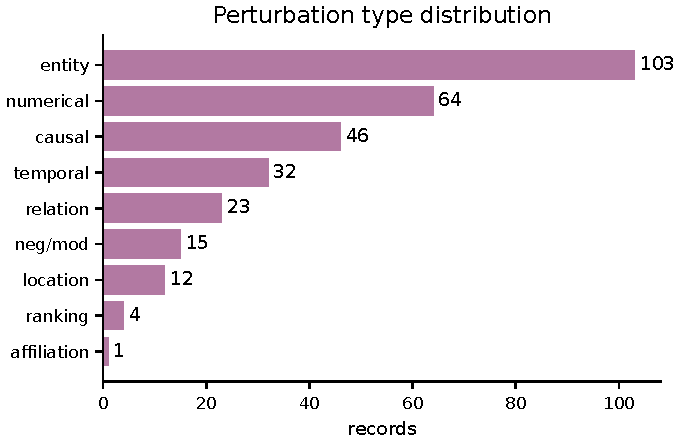
\includegraphics[width=\linewidth]{figures/type_distribution_large.pdf}
  \caption{Perturbation type distribution in the 300-record balanced set. Entity substitutions and numerical shifts dominate; relation inversions are rarer but behaviorally important.}
  \label{fig:type_distribution}
\end{figure}

\subsection{Raw-Data Audit}

The prior draft used repository markdown summaries. For this revision, we wrote and ran a new audit script over the JSONL files in \path{data/}: \path{data/exp/3provider_300.jsonl}, the three \path{05_label_eval.jsonl} files, and all nine \path{06_judge.jsonl} files. The script independently recomputes validation pass counts, provider composition, generator behavior counts, same-perturber affinity, validation-vs-gap effects, judge confusion matrices, F1/precision/recall, and localization metrics. It asserts the expected scale: 300 unique core records, 900 generator outputs, 897 LLM-labeled outputs, and 2,683 judge verdicts. The audit script and generated JSON are included in the source bundle.

\section{Generator and Judge Protocol}

\subsection{RAG Generation from Perturbed Grounding}

Each generator receives the original question and the perturbed grounding passages. The prompt instructs the model to answer using only the provided passages, cite passage IDs supporting factual claims, and refuse if the evidence is insufficient or inconsistent. We run three generator families over all 300 records, yielding 900 intended generator outputs and 897 successfully LLM-labeled outputs.

We distinguish six generator behaviors: \emph{context follow} (the answer asserts the perturbed value), \emph{memory override} (the answer asserts the original value), \emph{both claims}, \emph{conflict awareness}, \emph{refusal or insufficient evidence}, and \emph{unrelated or failed}. A separate LLM label-evaluation step assigns these labels paraphrase-aware; the deterministic string-match labeler is retained only as an audit signal.

\paragraph{Generation example.}
For the Caitlin Clark record, GPT is given perturbed passages stating a 35\% attendance jump. It answers: ``Caitlin Clark's 2024 WNBA debut/arrival was associated with a major jump in league attendance. Leaguewide attendance rose 35\% from 2023, reaching 2,353,735 total fans, the highest in 22 seasons. Her presence also boosted demand directly: her drafting alone resulted in higher game attendance, ticket sales increased by 93\%, and some teams moved Fever games to larger arenas.'' The label evaluator marks this \texttt{context\_follow} because the answer entails the perturbed value and not the original 48\% value. In contrast, for the Loschmidt record, GPT answers with the standard reversible-dynamics formulation even though the perturbed grounding altered the key value to ``irreversible''; that output is labeled \texttt{memory\_override}. Appendix~\ref{app:generation_examples} gives examples for context following, memory override, refusal, and conflict awareness.

\subsection{Blind Source-Grounded Judging}

For judging, each judge receives only the question, generated answer, and original grounding passages. It does not see the perturbed grounding, target value, replacement value, generator behavior labels, or gold induced-error label. The judge outputs a verdict, a boolean factual-error flag, the wrong claim if any, the most directly contradicting passage ID, an explanation, and confidence.

\noindent\begin{minipage}{\linewidth}
\paragraph{Judge output schema.}
The judge returns a structured JSON object:
\begin{lstlisting}
{
  "verdict": "correct | incorrect | unclear",
  "contains_factual_error": true | false,
  "wrong_claim": "string or null",
  "supporting_source_passage_id": "int or null",
  "explanation": "one or two sentences",
  "confidence": "high | medium | low"
}
\end{lstlisting}
\end{minipage}

The gold positive class is an induced factual error: a generator answer that entails the perturbed claim and should therefore be contradicted by the original grounding. We evaluate factual-error detection with precision, recall, and F1. We also evaluate localization: when a judge flags an error, does the cited source passage correspond to a passage modified by the perturbation, and does the extracted wrong claim contain the perturbed value?

\paragraph{Evaluation example.}
For the same Caitlin Clark question, a Gemini-generated answer says that league attendance jumped by 35\%. The Gemini judge, seeing the original passage, returns \texttt{incorrect}, sets \texttt{contains\_factual\_error=true}, identifies the wrong claim as ``Overall league attendance jumped by 35\%,'' and cites passage 1, where the original evidence states 48\%. This is a true positive in the Gemini-on-Gemini diagonal cell. Appendix~\ref{app:judge_examples} includes true positive, false negative, false positive, and true negative examples.

\paragraph{Model display names.}
The committed run artifacts contain deployment-specific identifiers. The main paper uses display labels GPT, Grok, and Gemini to avoid making claims depend on mutable proprietary deployment names; Appendix~\ref{app:repro} lists paths and version labels present in the repository.

\section{Results}

\subsection{Generators Often Trust Perturbed Evidence}

Figure~\ref{fig:generator_behavior} and Table~\ref{tab:gen_behaviors} show the audited LLM-labeled generator behavior distribution. All three generators accept the perturbed evidence frequently: context-follow rates are 51.2\% for GPT, 47.2\% for Grok, and 47.8\% for Gemini. By contrast, pure memory override is rare, at 1.3--3.3\%. This indicates that, under an instruction to use only the provided passages, models usually do not resist a coherent but false retrieved claim by substituting their parametric memory.

\begin{figure}[H]
  \centering
  
\includegraphics[width=\linewidth]{figures/generator_behavior_large.pdf}
  \caption{Generator behavior from the raw audit. Context following is the dominant induced-error source, while direct memory override is rare.}
  \label{fig:generator_behavior}
\end{figure}

\begin{table}[t]
\centering
\small
\begin{tabular}{lrrr}
\toprule
\textbf{Behavior label} & \textbf{GPT} & \textbf{Grok} & \textbf{Gemini} \\
\midrule
Context follow & 153 (51.2\%) & 141 (47.2\%) & 143 (47.8\%) \\
Memory override & 10 (3.3\%) & 8 (2.7\%) & 4 (1.3\%) \\
Both claims & 20 (6.7\%) & 15 (5.0\%) & 18 (6.0\%) \\
Conflict awareness & 3 (1.0\%) & 12 (4.0\%) & 4 (1.3\%) \\
Refusal/insufficient & 16 (5.4\%) & 74 (24.7\%) & 54 (18.1\%) \\
Unrelated/failed & 97 (32.4\%) & 49 (16.4\%) & 76 (25.4\%) \\
\bottomrule
\end{tabular}
\caption{Generator behavior labels over 897/900 LLM-labeled outputs. Percentages use the labeled denominator for each generator (299).}
\label{tab:gen_behaviors}
\end{table}

The non-context-follow mass differs by model. Grok refuses or declares insufficiency far more often than GPT, while GPT more often produces an answer that avoids the specific perturbed span. These answer styles later affect judge difficulty.

\subsection{Generator-Side Self-Affinity Is Not Uniform}

Before judging, we can ask whether a generator is more likely to follow perturbations created by its own family. GPT and Grok show positive self-affinity: GPT follows its own perturbations 56.6\% of the time compared with 49.1\% for other perturbations, and Grok follows its own 50.0\% compared with 45.9\% for others. Gemini reverses this pattern, following its own perturbations 46.0\% versus 49.1\% for others. This generator-side negative self-affinity foreshadows the judge-side result: Gemini is the model with the clearest self-skeptical signature.

\begin{figure}[H]
  \centering
  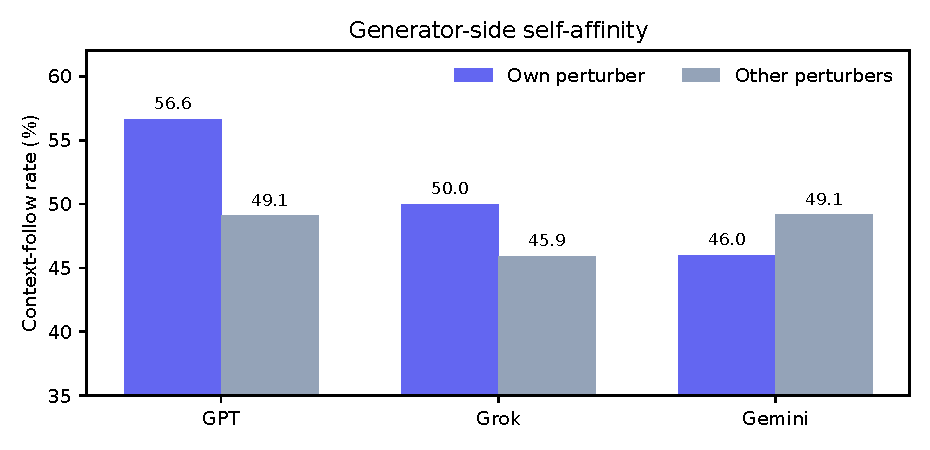
\includegraphics[width=\linewidth]{figures/generator_self_affinity.pdf}
  \caption{Generator-side self-affinity: context-follow rate for perturbations produced by the same family versus other families. Gemini is the only negative case.}
  \label{fig:self_affinity_gen}
\end{figure}

\begin{table}[t]
\centering
\small
\begin{tabular}{lrrr}
\toprule
\textbf{Generator} & \textbf{Own} & \textbf{Others} & \textbf{$\Delta$} \\
\midrule
GPT & 47/83 (56.6\%) & 106/216 (49.1\%) & +7.6\pp \\
Grok & 46/92 (50.0\%) & 95/207 (45.9\%) & +4.1\pp \\
Gemini & 57/124 (46.0\%) & 86/175 (49.1\%) & -3.2\pp \\
\bottomrule
\end{tabular}
\caption{Generator-side self-affinity: LLM-labeled context-follow rates for perturbations produced by the same family versus other families.}
\label{tab:self_affinity_gen}
\end{table}

\subsection{Judge Matrix: Strong but Uneven Error Detection}

Figure~\ref{fig:judge_matrix} and Table~\ref{tab:f1_matrix} show the headline judge-by-generator matrix. Across all nine cells, judges detect induced factual errors with F1 between 79.9\% and 88.6\%. The strongest judge row is Gemini, with an average F1 of 86.0\%. The strongest single cell is Gemini judging Gemini-generated answers, at 88.6\% F1.

\begin{figure}[H]
  \centering
  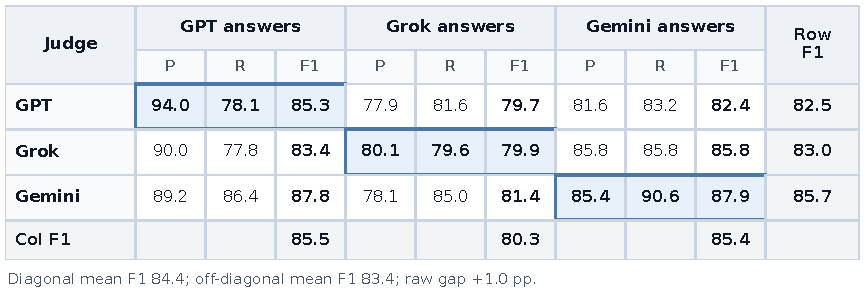
\includegraphics[width=\linewidth]{figures/judge_matrix_large.pdf}
  \caption{Audited blind factual-error detection matrix. Entries show F1 with precision and recall below. Asterisks mark diagonal cells.}
  \label{fig:judge_matrix}
\end{figure}

\begin{table*}[t]
\centering
\small
\begin{tabular}{lrrrr}
\toprule
 & \multicolumn{3}{c}{\textbf{Generator}} & \\
\cmidrule(lr){2-4}
\textbf{Judge} & \textbf{GPT} & \textbf{Grok} & \textbf{Gemini} & \textbf{Row avg.} \\
\midrule
GPT & \textbf{84.8}\%$^{\dagger}$ & 79.9\% & 83.6\% & 82.8\% \\
Grok & 83.4\% & \textbf{80.5}\%$^{\dagger}$ & 86.6\% & 83.5\% \\
Gemini & 87.5\% & 81.9\% & \textbf{88.6}\%$^{\dagger}$ & 86.0\% \\
\midrule
Column avg. & 85.3\% & 80.8\% & 86.2\% & 83.8\% \\
\bottomrule
\end{tabular}
\caption{F1 for factual-error detection in the full judge-by-generator matrix. $^{\dagger}$ marks same display-family diagonal cells. There are 296--300 verdicts per cell, 2,683 total.}
\label{tab:f1_matrix}
\end{table*}

The column averages reveal an important confound for judge studies: Grok-generated answers are harder for every judge to evaluate, with a column average of 80.8\% F1 compared with 85.3\% for GPT-generated and 86.2\% for Gemini-generated answers. This is consistent with Grok's much higher refusal rate and hedged style: judges must decide whether a refusal or insufficient-evidence answer is correct, rather than simply checking a crisp factual assertion.

\subsection{Same-Model Bias Is a Set of Signatures, Not a Scalar}

If we pool all diagonal cells and compare them with all off-diagonal cells, the same-model effect appears small: diagonal F1 averages 84.6\%, while off-diagonal F1 averages 83.8\%, a difference of +0.8\pp. This aggregate hides the main finding. Table~\ref{tab:bias_signatures} and Figure~\ref{fig:bias_signatures} show that the direction and mechanism differ by judge.

\begin{figure}[H]
  \centering
  
\includegraphics[width=\linewidth]{figures/same_model_deltas_large.pdf}
  \caption{Same-model deltas computed as each judge's diagonal cell minus its two off-diagonal cells. F1 deltas alone hide the recall mechanism: GPT's own recall drops, Gemini's own recall rises.}
  \label{fig:bias_signatures}
\end{figure}

\begin{table*}[t]
\centering
\small
\begin{tabularx}{\linewidth}{lrrrrY}
\toprule
\textbf{Judge} & \textbf{F1 own} & \textbf{F1 cross} & \textbf{Recall own} & \textbf{Recall cross} & \textbf{Signature} \\
\midrule
GPT & 84.8\% & 81.7\% & 77.5\% & 83.6\% & Higher own F1 but lower own recall: the GPT judge misses more induced errors in GPT outputs, a recall-lenient self pattern. \\
Grok & 80.5\% & 85.0\% & 80.5\% & 82.1\% & Own-cell degradation: Grok is worst on its own outputs, largely through lower precision and noisy verdicts. \\
Gemini & 88.6\% & 84.7\% & 91.5\% & 85.9\% & Higher own recall: Gemini catches more induced errors in Gemini outputs, a self-skeptical or anti-lenient pattern. \\
\bottomrule
\end{tabularx}
\caption{Per-judge same-model signatures. A pooled diagonal average masks opposing effects: GPT is self-lenient in recall, Gemini is self-strict in recall, and Grok degrades on self.}
\label{tab:bias_signatures}
\end{table*}

GPT's diagonal F1 is higher than its cross-generator average, but this is not because it catches more of its own errors. Its own-output recall is 6.2\pp lower than cross-output recall. Gemini exhibits the opposite pattern. It has both high same-model F1 and 5.6\pp higher same-model recall, meaning it catches more Gemini errors than cross-model errors. Grok does not show clean leniency or strictness; its own cell is simply weaker than its cross cells.

\subsection{Localization Is Reliable}

For downstream debugging, an error detector is more useful when it points to the contradicted source. Figure~\ref{fig:localization} summarizes the audited localization metrics. Across all matrix cells, the judge's supporting passage lies in the known modified passage set 94.0--98.5\% of the time for positive detections. The extracted wrong claim contains the perturbed value in 71.0--83.6\% of true-positive cases. Thus, citation localization is stronger than wrong-claim span extraction: judges are very good at pointing to the right source passage, but sometimes paraphrase the erroneous claim rather than repeating the perturbed value verbatim.

\begin{figure}[H]
  \centering
  
\includegraphics[width=\linewidth]{figures/localization_large.pdf}
  \caption{Localization metrics from the raw judge verdicts. Passage-level localization is consistently high; exact value containment is lower because wrong-claim text is often paraphrased.}
  \label{fig:localization}
\end{figure}

\section{Discussion}

\paragraph{Controlled perturbations turn judge bias into an error-detection problem.}
Preference-based judge studies must account for latent output quality. In our setup, a context-following answer is intentionally generated to be plausible under perturbed grounding but wrong under original grounding. This makes the positive class local, factual, and hidden from the judge. The result is a more direct test of whether a judge detects an error when the answer is fluent, cited, and possibly written by the same model family.

\paragraph{Do LLM judges favor themselves?}
The answer in this data is: sometimes, but not uniformly. GPT shows a self-lenient recall pattern. Gemini shows the opposite. Grok shows own-cell degradation without a clean leniency interpretation. Reporting only an average diagonal advantage would miss the central empirical structure. We recommend that RAG evaluation reports include a full judge-by-generator matrix whenever judges and generators overlap.

\paragraph{Generator behavior shapes judge evaluation.}
The hardest generator column is Grok, not because every judge fails on Grok in the same way, but because Grok produces many refusals and less direct factual claims. This suggests that judge robustness should be assessed across generator styles, not merely across judge models. A judge that performs well on direct factual answers may behave differently on refusals, hedges, or broad answers that avoid the perturbed claim.

\paragraph{Memory override is rare under coherent retrieval.}
The generator results support a secondary finding: when perturbed evidence is coherent and leakage is controlled, generators usually follow retrieval rather than override with pretraining knowledge. The memory-vs-retrieval conflict appears most clearly for relation inversions, where memory override and conflict awareness are much higher than for entity/date/number substitutions. This aligns with the intuition that some relational claims are more strongly encoded in parametric memory than arbitrary names or values.

\section*{Limitations}

This study is intentionally controlled and moderate scale. The balanced Phase-2 set contains 300 records, and the judge matrix contains 296--300 verdicts per cell; larger samples are needed to tighten confidence intervals for small same-model deltas. We evaluate one exact deployment per provider family, so the current matrix has no same-provider-different-model cells. Adding multiple models within the same family would separate exact-model effects from family-level style effects. The behavior-label gold signal is produced by an LLM label-evaluation step, not by exhaustive human annotation, although it is paraphrase-aware and grounded in explicit original/perturbed values. Judge calls are single-shot; rerunning judges would measure stochastic flip rates. Finally, the model versions are proprietary deployments and may change over time, so the qualitative finding--opposing same-model signatures--is more stable than any exact version-specific number.

\section*{Ethics Statement}

The benchmark is built from GaRAGe and generated perturbations of factual claims. The perturbations are designed for evaluation and should not be presented as factual information. The study does not evaluate people or make consequential decisions about individuals. The main risk is misuse of controlled misinformation generation; the pipeline mitigates this by retaining provenance, validation labels, and original/perturbed metadata for audit rather than releasing unlabeled corrupted passages as facts.

\section*{Reproducibility Statement}

The repository records the pipeline as JSONL artifacts and manifests. Core steps are \texttt{filter}, \texttt{perturb}, \texttt{validate}, \texttt{generate}, \texttt{label\_eval}, and \texttt{judge}. Each LLM call is traced with prompt, raw response, parsed JSON, tokens, latency, and run ID. For this revision, we include \path{audit/raw_data_audit.py}, \path{audit/audit_report.json}, and \path{audit/examples_report.json} in the source bundle. These recompute all central numbers from the raw JSONL files in \path{data/} and extract representative examples. Appendix~\ref{app:repro} lists the key commands and run artifacts used for this paper. All Graphviz DOT files and plotted vector figures are included in the source bundle.

\begin{thebibliography}{}

\bibitem[Bao et~al.(2024)]{bao2024faithbench}
Forrest Sheng Bao, Miaoran Li, Renyi Qu, Ge Luo, Erana Wan, Yujia Tang, Weisi Fan, Manveer Singh Tamber, Suleman Kazi, Vivek Sourabh, Mike Qi, Ruixuan Tu, Chenyu Xu, Matthew Gonzales, Ofer Mendelevitch, and Amin Ahmad. 2024.
\newblock FaithBench: A diverse hallucination benchmark for summarization by modern LLMs.
\newblock \emph{arXiv preprint arXiv:2410.13210}.

\bibitem[Dubois et~al.(2024)]{dubois2024length}
Yann Dubois, Bal{\'a}zs Galambosi, Percy Liang, and Tatsunori~B. Hashimoto. 2024.
\newblock Length-controlled AlpacaEval: A simple way to debias automatic evaluators.
\newblock \emph{arXiv preprint arXiv:2404.04475}.

\bibitem[Es et~al.(2023)]{es2023ragas}
Shahul Es, Jithin James, Luis Espinosa-Anke, and Steven Schockaert. 2023.
\newblock RAGAS: Automated evaluation of retrieval augmented generation.
\newblock \emph{arXiv preprint arXiv:2309.15217}.

\bibitem[Kim et~al.(2023)]{kim2023prometheus}
Seungone Kim, Jamin Shin, Yejin Cho, Joel Jang, Shayne Longpre, Hwaran Lee, Sangdoo Yun, Seongjin Shin, Sungdong Kim, James Thorne, and Minjoon Seo. 2023.
\newblock Prometheus: Inducing fine-grained evaluation capability in language models.
\newblock \emph{arXiv preprint arXiv:2310.08491}.

\bibitem[Lewis et~al.(2020)]{lewis2020rag}
Patrick Lewis, Ethan Perez, Aleksandra Piktus, Fabio Petroni, Vladimir Karpukhin, Naman Goyal, Heinrich K{\"u}ttler, Mike Lewis, Wen-tau Yih, Tim Rockt{\"a}schel, Sebastian Riedel, and Douwe Kiela. 2020.
\newblock Retrieval-augmented generation for knowledge-intensive NLP tasks.
\newblock In \emph{Advances in Neural Information Processing Systems}.

\bibitem[Liu et~al.(2023a)]{liu2023geval}
Yang Liu, Dan Iter, Yichong Xu, Shuohang Wang, Ruochen Xu, and Chenguang Zhu. 2023a.
\newblock G-Eval: NLG evaluation using GPT-4 with better human alignment.
\newblock \emph{arXiv preprint arXiv:2303.16634}.

\bibitem[Liu et~al.(2023b)]{liu2023lost}
Nelson~F. Liu, Kevin Lin, John Hewitt, Ashwin Paranjape, Michele Bevilacqua, Fabio Petroni, and Percy Liang. 2023b.
\newblock Lost in the middle: How language models use long contexts.
\newblock \emph{Transactions of the Association for Computational Linguistics}.

\bibitem[Liu et~al.(2024)]{liu2024narcissistic}
Yiqi Liu, Nafise Sadat Moosavi, and Chenghua Lin. 2024.
\newblock LLMs as narcissistic evaluators: When ego inflates evaluation scores.
\newblock In \emph{Findings of the Association for Computational Linguistics: ACL}.

\bibitem[Manakul et~al.(2023)]{manakul2023selfcheckgpt}
Potsawee Manakul, Adian Liusie, and Mark J.~F. Gales. 2023.
\newblock SelfCheckGPT: Zero-resource black-box hallucination detection for generative large language models.
\newblock \emph{arXiv preprint arXiv:2303.08896}.

\bibitem[Niu et~al.(2023)]{niu2023ragtruth}
Cheng Niu, Yuanhao Wu, Juno Zhu, Siliang Xu, Kashun Shum, Randy Zhong, Juntong Song, and Tong Zhang. 2023.
\newblock RAGTruth: A hallucination corpus for developing trustworthy retrieval-augmented language models.
\newblock \emph{arXiv preprint arXiv:2401.00396}.

\bibitem[Saad-Falcon et~al.(2023)]{saadfalcon2023ares}
Jon Saad-Falcon, Omar Khattab, Christopher Potts, and Matei Zaharia. 2023.
\newblock ARES: An automated evaluation framework for retrieval-augmented generation systems.
\newblock \emph{arXiv preprint arXiv:2311.09476}.

\bibitem[Shi et~al.(2024)]{shi2024position}
Lin Shi, Chiyu Ma, Wenhua Liang, Weicheng Ma, and Soroush Vosoughi. 2024.
\newblock Judging the judges: A systematic study of position bias in LLM-as-a-judge.
\newblock \emph{arXiv preprint arXiv:2406.07791}.

\bibitem[Sorodoc et~al.(2025)]{sorodoc2025garage}
Ionut-Teodor Sorodoc, Leonardo F.~R. Ribeiro, Rexhina Blloshmi, Christopher Davis, and Adri{\`a} de Gispert. 2025.
\newblock GaRAGe: A benchmark with grounding annotations for RAG evaluation.
\newblock \emph{arXiv preprint arXiv:2506.07671}.

\bibitem[Spiliopoulou et~al.(2025)]{spiliopoulou2025playfavorites}
Evangelia Spiliopoulou, Riccardo Fogliato, Hanna Burnsky, Tamer Soliman, Jie Ma, Graham Horwood, and Miguel Ballesteros. 2025.
\newblock Play favorites: A statistical method to measure self-bias in LLM-as-a-judge.
\newblock \emph{arXiv preprint arXiv:2508.06709}.

\bibitem[Wataoka et~al.(2024)]{wataoka2024selfpreference}
Koki Wataoka, Tsubasa Takahashi, and Ryokan Ri. 2024.
\newblock Self-preference bias in LLM-as-a-judge.
\newblock \emph{arXiv preprint arXiv:2410.21819}.

\bibitem[Ye et~al.(2024)]{ye2024justice}
Jiayi Ye, Yanbo Wang, Yue Huang, Dongping Chen, Qihui Zhang, Nuno Moniz, Tian Gao, Werner Geyer, Chao Huang, Pin-Yu Chen, Nitesh~V. Chawla, and Xiangliang Zhang. 2024.
\newblock Justice or prejudice? Quantifying biases in LLM-as-a-judge.
\newblock \emph{arXiv preprint arXiv:2410.02736}.

\bibitem[Zheng et~al.(2023)]{zheng2023judging}
Lianmin Zheng, Wei-Lin Chiang, Ying Sheng, Siyuan Zhuang, Zhanghao Wu, Yonghao Zhuang, Zi Lin, Zhuohan Li, Dacheng Li, Eric~P. Xing, Hao Zhang, Joseph~E. Gonzalez, and Ion Stoica. 2023.
\newblock Judging LLM-as-a-judge with MT-Bench and Chatbot Arena.
\newblock \emph{arXiv preprint arXiv:2306.05685}.

\end{thebibliography}

\appendix

\section{Audit Implementation}
\label{app:audit}

The revision audit script independently recomputes the paper numbers from raw data files, not from repository markdown summaries. It checks: \texttt{data/exp/3provider\_300.jsonl}; the three generation/label-evaluation files \path{data/runs/20260531-005101-gen-gpt55-300/05_label_eval.jsonl}, \path{data/runs/20260531-005112-gen-grok-300/05_label_eval.jsonl}, and \path{data/runs/20260531-005123-gen-gemini-300/05_label_eval.jsonl}; and the nine judge files under \path{data/runs/20260531-*judge-*}. The script asserts 300 unique core records, 900 generator outputs, 897 LLM-labeled outputs, 2,683 judge verdicts, and pair types limited to same-exact-model and cross-provider-family. The source bundle includes the script and generated audit JSON.

\begin{figure*}[h]
  \centering
  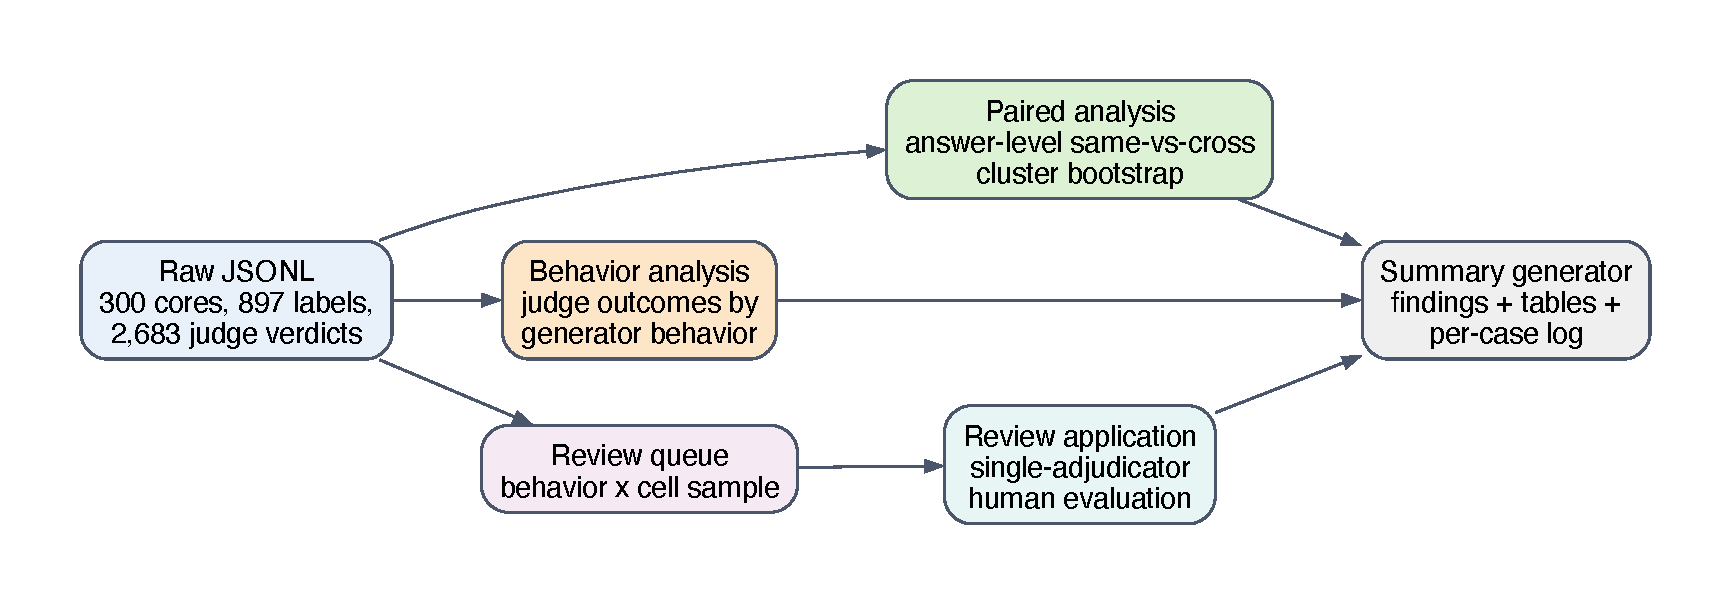
\includegraphics[width=0.93\linewidth]{figures/audit_flow.pdf}
  \caption{Raw-data audit flow used for this revision. All tables and visualizations are derived from \texttt{audit\_report.json}, which is generated from raw JSONL files.}
  \label{fig:audit_flow}
\end{figure*}

\section{Perturbation and Validation Examples}
\label{app:examples}

\begin{table*}[h]
\centering
\scriptsize
\begin{tabularx}{\linewidth}{L{1.15cm}L{1.25cm}L{2.9cm}L{1.8cm}Y Y}
\toprule
\textbf{Example} & \textbf{Type} & \textbf{Question} & \textbf{Value swap} & \textbf{Perturbed passage snippet} & \textbf{Validation gates} \\
\midrule
numeric & number & How did Caitlin Clark's WNBA debut influence league attendance in 2024? & 48\% $\rightarrow$ 35\% & In her rookie WNBA season, the league saw a 35\% jump in attendance from 2023. The league's total attendance of 2,353,735 was the highest in 22 seasons. & type valid=true, answer causal=true, global context consistent=true, no original answer leakage=true, original contradicts perturbed=true \\
relation & relation & What were the outcomes of the initial Zantac trials involving Abbott and Mead Johnson? & defense verdict $\rightarrow$ plaintiff verdict & The plaintiff verdict in Whitfield v. Abbott is a devastating loss for Abbott and Reckitt, Mead Johnson's parent--whose share prices plummeted significantly after the news. & type valid=true, answer causal=true, global context consistent=true, no original answer leakage=true, original contradicts perturbed=true \\
gap-fill & number & What are the expected benefits and risks of Ethereum 2.0 for long-term investors? & two $\rightarrow$ seventeen & Ethereum's upcoming Pectra upgrade in 2025 is met with optimism, as seventeen out of its 19 upgrades historically generated notable price impacts. & type valid=false, answer causal=false, global context consistent=true, no original answer leakage=false, original contradicts perturbed=true \\
\bottomrule
\end{tabularx}
\caption{Representative perturbation records extracted from the raw JSONL data. The gap-fill example is intentionally retained with explicit failed validation gates.}
\end{table*}

\section{Generation Examples}
\label{app:generation_examples}

\begin{table*}[h]
\centering
\scriptsize
\begin{tabularx}{\linewidth}{L{1.35cm}L{1.45cm}L{2.9cm}L{1.8cm}Y Y}
\toprule
\textbf{Example} & \textbf{Behavior} & \textbf{Question} & \textbf{Swap} & \textbf{Generator answer snippet} & \textbf{Label rationale} \\
\midrule
context follow & context follow & How did Caitlin Clark's WNBA debut influence league attendance in 2024? & 48\% $\rightarrow$ 35\% & Caitlin Clark's 2024 WNBA debut/arrival was associated with a major jump in league attendance. Leaguewide attendance rose 35\% from 2023, reaching 2,353,735 total fans, the highest in 22 seasons. Her presence also boosted demand directly: her drafting alone resulted in higher game attendance, ticket sales increased by 93\%, and some teams moved Fever games to larger arenas. & The answer explicitly states that leaguewide attendance rose 35\% from 2023, matching the perturbed passages. It does not mention or imply the original 48\% figure. \\
memory override & memory override & How does Loschmidt's paradox challenge Boltzmann's H theorem? & reversible $\rightarrow$ irreversible & Loschmidt's paradox challenges Boltzmann's H-theorem by arguing that one should not be able to derive an irreversible increase of entropy from underlying time-symmetric or microscopically reversible dynamics. & The answer states the standard formulation that Loschmidt's paradox objects to deriving macroscopic irreversibility from time-symmetric or microscopically reversible dynamics, contradicting the perturbed documents' altered claim. \\
refusal & refusal & How has Letsile Tebogo's cultural heritage influenced his athletic career? & Botswana $\rightarrow$ Ghana & The provided passages do not contain sufficient information on how Letsile Tebogo's cultural heritage has influenced his athletic career. & The answer explicitly states that the passages do not provide sufficient information and declines to assert how Tebogo's cultural heritage influenced his career. \\
conflict aware & conflict aware & What impact has National Dog Month had on dog adoption rates? & promotes pet adoption $\rightarrow$ discourages pet adoption & The passages do not provide a clear, evidence-based adoption-rate impact specifically for National Dog Month, so I can't answer that directly. They only say National Dog Month promotes adoption and raises awareness of rescue dogs, while other passages inconsistently claim it discourages adoption. & The answer explicitly says the evidence is inconsistent, noting some passages say National Dog Month promotes adoption while others say it discourages adoption. \\
\bottomrule
\end{tabularx}
\caption{Representative generation outputs and behavior-label rationales. These examples illustrate why paraphrase-aware LLM labels were used instead of publication claims based on strict string matching.}
\end{table*}

\section{Judge Output Schema and Examples}
\label{app:judge_examples}

\begin{lstlisting}
{
  "judge_provider": "azure-gpt | grok | gemini",
  "judge_model": "exact deployment id",
  "generator_provider": "azure-gpt | grok | gemini",
  "generator_model": "exact deployment id",
  "generator_mode": "rag_perturbed",
  "pair_type": "same_exact_model | same_provider_family | cross_provider_family",
  "verdict": "correct | incorrect | unclear",
  "contains_factual_error": true | false,
  "wrong_claim": "string or null",
  "supporting_source_passage_id": 3,
  "explanation": "one or two sentences",
  "confidence": "high | medium | low",
  "gold_has_induced_error": true,
  "gold_perturbation_target": "original value",
  "gold_perturbation_replacement": "perturbed value"
}
\end{lstlisting}

\begin{table*}[h]
\centering
\scriptsize
\begin{tabularx}{\linewidth}{L{1.0cm}L{1.45cm}L{0.9cm}L{0.9cm}L{2.8cm}Y Y}
\toprule
\textbf{Example} & \textbf{Cell} & \textbf{Gold} & \textbf{Pred.} & \textbf{Question} & \textbf{Wrong claim} & \textbf{Judge explanation} \\
\midrule
TP same & Gemini/Gemini & True & True & How did Caitlin Clark's WNBA debut influence league attendance in 2024? & Overall league attendance jumped by 35\% compared to 2023, reaching a total of 2,353,735, which was the highest in 22 seasons. & The answer incorrectly claims a 35\% increase in overall league attendance, while the source passages state it jumped by 48\%. \\
FN & GPT/GPT & True & False & How does RL contribute to personalized learning experiences in education? &  & The answer is supported by the passages: RL adapts learning using student interactions and performance over time, tailors content/pacing/feedback to individual needs, and can adjust assessments in real time. \\
FP & Grok/GPT & False & True & How have recent SEC changes affected operating lease reporting practices? & Under ASC 842, companies must recognize most leases--including operating leases--on the balance sheet. & Passage 2 attributes ASC 842 to FASB rather than SEC, and no source links SEC rule changes to the specific balance-sheet recognition requirements. \\
TN & GPT/Grok & False & False & How has Letsile Tebogo's cultural heritage influenced his athletic career? &  & The passages mention Letsile Tebogo as Botswana's sprinting star and discuss Botswana's sports culture generally, but they do not explain how his own cultural heritage influenced his athletic career. \\
\bottomrule
\end{tabularx}
\caption{Representative judge outcomes: true positive, false negative, false positive, and true negative. Gold is the hidden induced-error label; Pred. is the judge's \texttt{contains\_factual\_error}.}
\end{table*}

\section{Additional Data Visualizations}
\label{app:extra_figs}

\begin{figure*}[h]
  \centering
  
\includegraphics[width=0.95\linewidth]{figures/type_by_provider_heatmap.pdf}
  \caption{Perturbation type by selected perturber in the balanced set. This highlights model-specific perturbation preferences: GPT contributes many causal changes, Grok many entity/numerical substitutions, and Gemini many entity substitutions and relation inversions.}
\end{figure*}

\begin{figure*}[h]
  \centering
  \begin{subfigure}{0.48\linewidth}
    
\includegraphics[width=\linewidth]{figures/validated_vs_gap.pdf}
    \caption{Context-following on validated vs gap-fill records.}
  \end{subfigure}
  \hfill
  \begin{subfigure}{0.48\linewidth}
    
\includegraphics[width=\linewidth]{figures/relation_pushback.pdf}
    \caption{Relation inversion pushback.}
  \end{subfigure}
  \caption{Additional generator behavior analyses. Gap-fill records still affect generators, and relation inversions uniquely expose memory-vs-retrieval tension.}
\end{figure*}

\begin{figure*}[h]
  \centering
  
\includegraphics[width=0.88\linewidth]{figures/confusion_counts.pdf}
  \caption{Confusion counts per judge-generator cell. The matrix shows that the Grok-generator column is harder across judges and that diagonal behavior differs by judge.}
\end{figure*}

\section{Perturbation Type Distribution}
\label{app:types}

\begin{table}[h]
\centering
\small
\begin{tabular}{lrr}
\toprule
\textbf{Type} & \textbf{Count} & \textbf{Share} \\
\midrule
Entity substitution & 103 & 34.3\% \\
Numerical shift & 64 & 21.3\% \\
Causal change & 46 & 15.3\% \\
Temporal shift & 32 & 10.7\% \\
Relation inversion & 23 & 7.7\% \\
Negation/modality & 15 & 5.0\% \\
Location change & 12 & 4.0\% \\
Ranking flip & 4 & 1.3\% \\
Affiliation change & 1 & 0.3\% \\
\bottomrule
\end{tabular}
\caption{Perturbation type distribution in the audited balanced 300-record dataset.}
\end{table}

\begin{table}[h]
\centering
\small
\begin{tabular}{lrrr}
\toprule
\textbf{Generator} & \textbf{$n$} & \textbf{Memory override} & \textbf{Conflict awareness} \\
\midrule
GPT & 23 & 17.4\% & 4.3\% \\
Grok & 23 & 17.4\% & 21.7\% \\
Gemini & 23 & 13.0\% & 13.0\% \\
\bottomrule
\end{tabular}
\caption{Relation inversion is small in count but has much higher memory-override and conflict-awareness rates than most other perturbation types.}
\end{table}

\section{Full Judge Metrics}
\label{app:full_judge}

\begin{table*}[h]
\centering
\scriptsize
\begin{tabular}{llrrrrrrrrr}
\toprule
\textbf{Judge} & \textbf{Gen.} & \textbf{$n$} & \textbf{Gold +} & \textbf{TP} & \textbf{FP} & \textbf{FN} & \textbf{TN} & \textbf{Prec.} & \textbf{Rec.} & \textbf{F1} \\
\midrule
GPT & GPT & 297 & 173 & 134 & 9 & 39 & 115 & 93.7 & 77.5 & 84.8 \\
GPT & Grok & 299 & 159 & 131 & 38 & 28 & 102 & 77.5 & 82.4 & 79.9 \\
GPT & Gemini & 296 & 165 & 140 & 30 & 25 & 101 & 82.4 & 84.8 & 83.6 \\
Grok & GPT & 299 & 175 & 136 & 15 & 39 & 109 & 90.1 & 77.7 & 83.4 \\
Grok & Grok & 300 & 159 & 128 & 31 & 31 & 110 & 80.5 & 80.5 & 80.5 \\
Grok & Gemini & 296 & 164 & 142 & 22 & 22 & 110 & 86.6 & 86.6 & 86.6 \\
Gemini & GPT & 299 & 175 & 151 & 19 & 24 & 105 & 88.8 & 86.3 & 87.5 \\
Gemini & Grok & 300 & 159 & 136 & 37 & 23 & 104 & 78.6 & 85.5 & 81.9 \\
Gemini & Gemini & 297 & 165 & 151 & 25 & 14 & 107 & 85.8 & 91.5 & 88.6 \\
\bottomrule
\end{tabular}
\caption{Full audited confusion counts and metrics for all nine cells. Metrics are percentages.}
\end{table*}

\begin{table*}[h]
\centering
\small
\begin{tabular}{lrrrrrr}
\toprule
 & \multicolumn{3}{c}{\textbf{Citation locality}} & \multicolumn{3}{c}{\textbf{Wrong-claim contains replacement}} \\
\cmidrule(lr){2-4}\cmidrule(lr){5-7}
\textbf{Judge} & \textbf{Gen=GPT} & \textbf{Gen=Grok} & \textbf{Gen=Gemini} & \textbf{Gen=GPT} & \textbf{Gen=Grok} & \textbf{Gen=Gemini} \\
\midrule
GPT & 94.0 & 95.4 & 95.0 & 75.4 & 71.0 & 83.6 \\
Grok & 98.4 & 98.3 & 98.5 & 76.5 & 74.2 & 82.4 \\
Gemini & 95.3 & 95.5 & 97.3 & 76.8 & 72.8 & 81.5 \\
\bottomrule
\end{tabular}
\caption{Localization quality across matrix cells. Citation locality is consistently higher than exact replacement containment in the wrong-claim field.}
\end{table*}

\section{Run Artifacts and Reproducibility}
\label{app:repro}

The following repository artifacts are the primary evidence for the paper.

\begin{itemize}[leftmargin=*]
  \item \textbf{Balanced dataset:} \path{data/exp/3provider_300.jsonl} and \path{data/exp/3provider_300.manifest.json}.
  \item \textbf{Perturb/validate full runs:} \path{20260530-183135-300q-gpt-full}, \path{20260530-183144-300q-grok-full}, and \path{20260530-183151-300q-gemini-full} under \path{data/runs/}.
  \item \textbf{Generation runs:} \path{20260531-005101-gen-gpt55-300}, \path{20260531-005112-gen-grok-300}, and \path{20260531-005123-gen-gemini-300} under \path{data/runs/}.
  \item \textbf{Judge runs:} judge-on-GPT, judge-on-Grok, and judge-on-Gemini directories under \path{data/runs/20260531-*}.
\end{itemize}

The canonical high-level rebuild sequence is: fetch GaRAGe; build \path{exp-300} with \texttt{--n 300}; run three full perturb/validate pipelines over the frozen pool; build \path{3provider_300} with \texttt{build-balanced --target 300 --seed 17}; generate answers with GPT, Grok, and Gemini; run \texttt{label-eval}; and finally run the nine judge cells. The run metadata uses deployment-specific labels. The main text reports display labels to avoid making claims depend on mutable proprietary deployment names; exact provider/model IDs remain in the JSONL \texttt{generators} and \texttt{judge\_verdicts} provenance fields.

\end{document}
